\documentclass[11pt]{article}\usepackage[left=20mm,right=20mm,top=15mm,bottom=20mm]{geometry}

\usepackage[T1]{fontenc}
\usepackage[magyar]{babel}
\usepackage[utf8]{inputenc}
\usepackage[table,xcdraw]{xcolor}

\usepackage{graphicx}
\usepackage{caption}
\usepackage{siunitx}
\usepackage{amsmath}
\usepackage{epstopdf}
\usepackage{multirow}
\usepackage{makeidx}
\usepackage[]{mcode}
\usepackage{placeins}
\usepackage{subcaption}
\usepackage{hyperref}

%\DeclareUnicodeCharacter{00A0}{~}

\begin{document}
\begin{titlepage}
\centering
	
\includegraphics[width=0.5\textwidth]{figures/bme_logo_kicsi.eps}\par\vspace{1cm}
	\vspace{1cm}
	\vspace{1.5cm}
	{\huge\bfseries Szoftvertervezés 1. házi feladat \par}
	\vspace{15cm}
	{\huge\itshape Locskai Norbert, Kovács András, Barancsuk Lilla \par}
	\vfill

% Bottom of the page
	{\large \today\par}
\end{titlepage}

\section{Vízió}

\begin{table}[]
\centering
\label{tab:vizio_fejlec}
\begin{tabular}{|l|l|l|l|}
\hline
\rowcolor[HTML]{EFEFEF} 
\multicolumn{1}{|c|}{\cellcolor[HTML]{EFEFEF}\textbf{Verzió}} & \multicolumn{1}{c|}{\cellcolor[HTML]{EFEFEF}\textbf{Dátum}} & \multicolumn{1}{c|}{\cellcolor[HTML]{EFEFEF}\textbf{Leírás}} & \multicolumn{1}{c|}{\cellcolor[HTML]{EFEFEF}\textbf{Készítő}}             \\ \hline
Első verzió                                                   & \today                                                      & Vízió kész                                                   & \begin{tabular}[c]{@{}l@{}}Locskai Norbert\\ Barancsuk Lilla\end{tabular} \\ \hline
                                                              &                                                             &                                                              &                                                                           \\ \hline
\end{tabular}
\end{table}

\subsection{Bevezetés}
A Service4U cég berendezések szervizelésével foglalkozik. Az Device4U nemzetközi cég által
gyártott berendezések szervizelését végzi Magyarországon.
A Service4U vezetői egy olyan számítógépes rendszert szeretnének, mely segítségével képesek
lesznek a raktárban tárolt alkatrész készletet nyomon követni, a rendelés, felhasználás, szállítás, ill.
leltározás folyamatait támogatni.

\subsubsection{Megoldandó probléma}
A programnak nyilván kell tartania a raktárban található összes alkatrészt, illetve azokat az időpontokat, amikor a raktár tartalma változott, a változást, illetve azt, aki a változást bevitte a rendszerbe, valamint segítenie kell a rendelések összeállítását.

Emiatt a rendszernek nyilván kell tartania a cég azon dolgozóit is, akik a programot használják (a vezetőség tagjait, illetve a raktárosokat, akik a rendeléseket átveszik, és az eszközöket kiadják).

A program segítségével a cég vezetőinek képesnek kell lenniük rendelések összeállítására, illetve azok exportálására többféle formátumban (pdf, xls, txt).
 
Mivel a Service4U minden alkatrészből legalább két darabot kíván raktáron tartani, a programnak értesítenie kell a cég vezetőségét, amennyiben bármely alkatrész száma kettő alá csökken.

Az alkatrészeket a Service4U cég szerelői vételezik ki a raktárból egy-egy berendezés javítása
során. 
A szerelők a kivenni kívánt alkatrészeket munkalapon rögzítik, amjd azt átadják a raktárosnak. 
A raktárosnak a rendszer segítségével képesnek kell lennie a kivétel nyilvántartására: az időpont, a szerelő, a raktáros azonosítójának, illetve a kivett alkatrészek rögzítésére.

A szállítást mindig azonos szállító cég végzi, akik adott rendelést mindig egy szállítási egységként szállítják.
A program segítségével a raktá

Service4U cég vezető félévente leltározást végeznek a raktárban, amikor elkészítik azt a listát, ami a
raktárban levő alkatrészek listáját tartalmazza.
A Device4U viszonylak kevés különböző berendezést gyárt és azok évente változnak, azonos
alkatrészeket tartalmaznak, egy-egy berendezés sok alkatrészből állhat.

\subsection{Érdekeltek köre - stakeholderek + céljaik}
\begin{itemize}
\item[] \textbf{szerelő} :A szerelő az, aki végzi a gépek javítását. A rendszer segítségével szeretné meggyorsítani az elvégzett munka dokumentálását. (Mennyi alkatrészt használt fel.)
\item[] \textbf{raktáros}
\item[] \textbf{rendszergazda}
\item[] \textbf{vezető} Ő viszi be az új alkatrészeket is.
\end{itemize}

\subsection{Rendszer részei}
\begin{itemize}
\item[] \textbf{adatbázis}: nyilvántartás
\item[] \textbf{köztes rész}: adatbázist és grafikus felületet összekötő interfész
\item[] \textbf{GUI}
\item[] \textbf{azonosítófelület}
\item[] \textbf{lehetőség távoli hozzáférésre} (helyi hálózat, internet)
\item[] \textbf{vonalkódleolvasó} - vonalkódfeldolgozó
\end{itemize}

\subsection{Rendszer korlátai, határai}
\subsubsection{Mit nem csinál?}
Nem automatizált a raktár feltöltése-ürítése, leltározás, raktáros csinálja.
Kollégák nyilvántartását nem veszi át automatikusan a céges rendszerből, kézzel kell bevinni az azonosítójukat.
Nem a rendszer feladata a rendelés elküldése, csak generálása.

\subsubsection{Technológiai korlátok}
Egy szerver van, mindenki böngészőn keresztül lép be...
(Autentikáció nem kell helyi gépről)


\section{Fogalomszótár - glossary}
\begin{itemize}
\item[]\textbf{berendezés}
\item[]\textbf{alkatrész}
\item[]\textbf{szerelő}
\item[]\textbf{cégvezető}
\item[]\textbf{raktáros}
\item[]\textbf{szállítólevél}
\item[]\textbf{munkalap}
\item[]\textbf{rendszergazda}
\item[]\textbf{rendelés}
\item[]\textbf{leltározás}
\item[]\textbf{jelentés}
\end{itemize}

\section{Kiegészítő követelmények leírása - supplementary specification}

\begin{table}[]
\centering
\label{tab:srs_fejlec}
\begin{tabular}{|l|l|l|l|}
\hline
\rowcolor[HTML]{EFEFEF} 
\multicolumn{1}{|c|}{\cellcolor[HTML]{EFEFEF}\textbf{Verzió}} & \multicolumn{1}{c|}{\cellcolor[HTML]{EFEFEF}\textbf{Dátum}} & \multicolumn{1}{c|}{\cellcolor[HTML]{EFEFEF}\textbf{Leírás}} & \multicolumn{1}{c|}{\cellcolor[HTML]{EFEFEF}\textbf{Készítő}}             \\ \hline
Első verzió                                                   & \today                                                      & Vízió kész                                                   & \begin{tabular}[c]{@{}l@{}}Locskai Norbert\\ Barancsuk Lilla\end{tabular} \\ \hline
                                                              &                                                             &                                                              &                                                                           \\ \hline
\end{tabular}
\end{table}

\subsection{Bevezetés}
Röviden a rendszer célja, ezért kell, hogy a rendszer...

\subsection{Usability}
GUI egyszerű, ergonomikus

\subsection{Reliability}
Backlog az adatbázisban, rendszeres mentés, követhető, hogy
ki mikor mit csinált. Visszaállíthatóság. 
Munkanapokon éjfélkor készül egy biztonsági mentés,

\subsection{Performance}
Sok alkatrész: max 1000 féle alkatrészt tárol, max 1000 db mindegyikből. Rendszer max 500 féle gép alkatrészeit ismeri. Egy gép max 200 alkatrszéből állhat. Egyszerre max 10-en férhetnek hozzá a rendszerhez. 

\subsection{Supportability}
Adatbázis bővíthető legyen, grafikus interfész tetszőlegesen változtatható a használt böngésző korlátai között.
A cég vállalja a rendszeres karbantartást. (félévente randszeresen, igény szerint - telefonos support)

\subsection{Implementation constraints}
Legelterjedtebb böngészőkön (Safari, Chrome, Mozzilla, IE) működik.
Céges PC-k. (szar az összes... korlátozott proci, memóia) Céges szerver: ... (ez is szar)
Vonalkódleolvasó

\subsection{Interfaces}
Nem szükséges ilyennel együttműködni.

\section{Use Case modell}
\subsection{Aktorok}
\subsubsection{Elsődleges}
\subsubsection{Támogató}
\subsection{Háttér}

\subsection{User nyilvántartás}
rendszergazda

\subsection{Bejelentkezés}
raktáros, rendszergazda, vezetől

\subsection{Rendelés}
- azonosító : UC1
- aktorok: 
- stakeholderek:
- előfeltételek:
- hatása: postconditions
- basic flow:
- alternative flow:
- special requirements
- technology and data variations list.... 
- open issues
előfeltételek: ha 2-nél kevesebb van egy alkatrészből mindenképpen, de lehet enélkül is

\begin{figure}[!h]
    \centering
        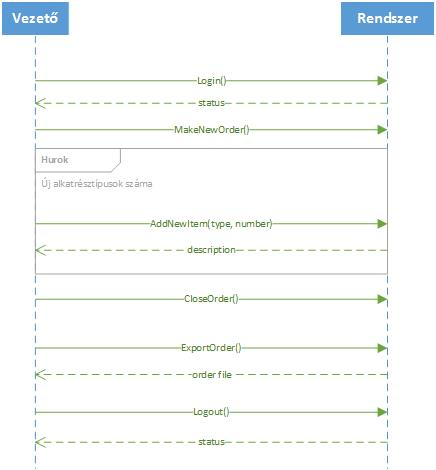
\includegraphics[width=0.9\textwidth]{figures/rendeles_SD.jpg}
        \caption{A rendelés szekvenciadiagramja.}
\end{figure}

\begin{figure}[!h]
    \centering
        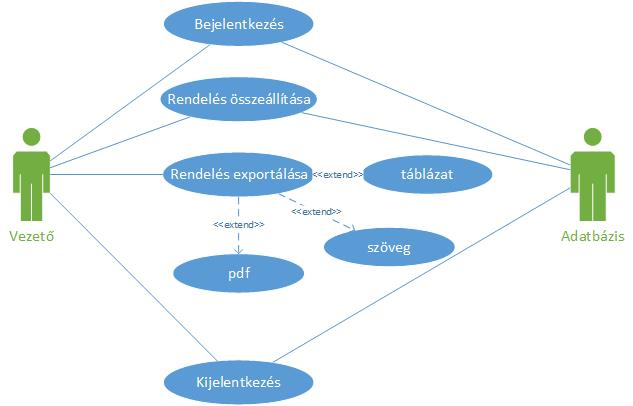
\includegraphics[width=0.9\textwidth]{figures/rendeles_UC.jpg}
        \caption{A rendelés use case diagramja.}
\end{figure}

\subsection{Automatikus értesítés}
vezetőknek, ha nincs elég egy alkatrészből

\subsection{Új gép bevitele}
vezetők

\subsection{Backlog lekérdezése}
vezetők

\subsection{Leltárazás}
- azonosító : UC2
- aktorok: A leltárazásban részt vesz a cégvezetés... Mit csinál?
- stakeholderek: Raktárosok számolják össze, hogy mennyi van...
- előfeltételek:
- hatása: postconditions
- basic flow:
- alternative flow:
- special requirements
- technology and data variations list.... 
- open issues
vezetők

\begin{figure}[!h]
    \centering
        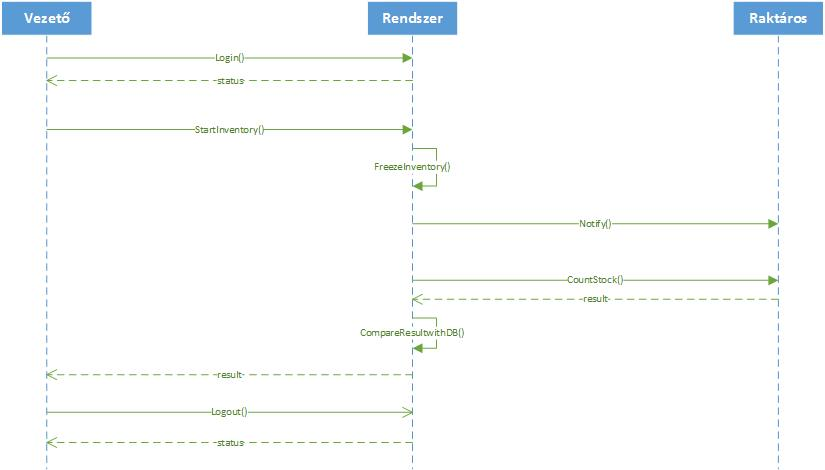
\includegraphics[width=0.9\textwidth]{figures/leltarazas_SD.jpg}
        \caption{A leltározás szekvenciadiagramja.}
\end{figure}

\begin{figure}[!h]
    \centering
        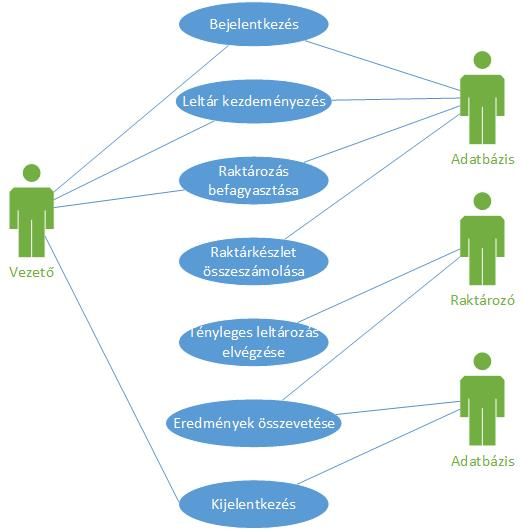
\includegraphics[width=0.9\textwidth]{figures/leltarazas_UC.jpg}
        \caption{A leltározás use case diagramja.}
\end{figure}

\subsection{Megrendelés átvétele}
raktáros

\subsection{Alkatrész kiadása}
- azonosító : UC3
- aktorok: 
- stakeholderek:
- előfeltételek:
- hatása: postconditions
- basic flow:
- alternative flow:
- special requirements
- technology and data variations list.... 
- open issues

\begin{figure}[!h]
    \centering
        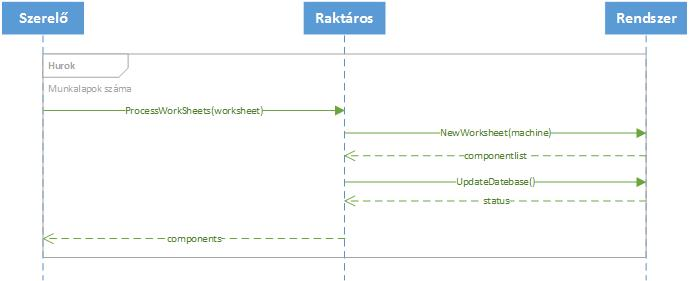
\includegraphics[width=0.9\textwidth]{figures/alkatresz_kiadas_SD.jpg}
        \caption{Az alkatrész kiadás szekvenciadiagramja.}
\end{figure}

\begin{figure}[!h]
    \centering
        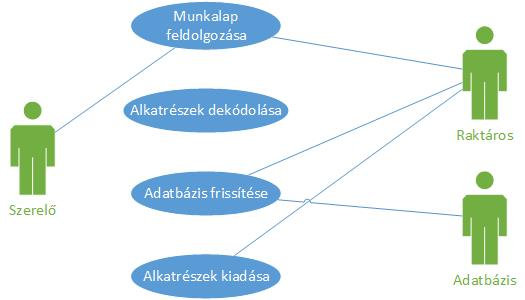
\includegraphics[width=0.9\textwidth]{figures/alkatresz_kiadas_UC.jpg}
        \caption{Az alkatrész kiadás use case diagramja.}
\end{figure}

\subsection{Biztonsági mentés készítése}
timer csinálja

\subsection{Rendszer visszaállítása}
rendszergazda kezdeményezi





\FloatBarrier
\end{document}